%%%%%%%%%%%%%%%%%%%%%%%%
%
%   Thesis template by Youssif Al-Nashif
%
%   May 2020
%
%%%%%%%%%%%%%%%%%%%%%%%%

\section{Hierarchical Clustering}


\subsection{NHTSA Special Crash Investigations}
 For the NHTSA's Special Crash Investigation dataset, a hierarchical clustering was performed on the resulting graph kernel computed from the skip-gram graphs. Since this dataset was pretty small at $N=48$, it served as a good subject to study the interactions between modifying the skip window width, kernel hyper parameters, and number of clusters. This study on these interactions informs decisions made on which hyper parameters to use in final analysis of the NHTSA data as well as the reddit thread data. \\
 
For the study on these interactions, hyper-parameters were varied and the value of cluster within sum of squares was tracked. Specifically, the values in Figure X were tested. \\
 

\begin{figure}
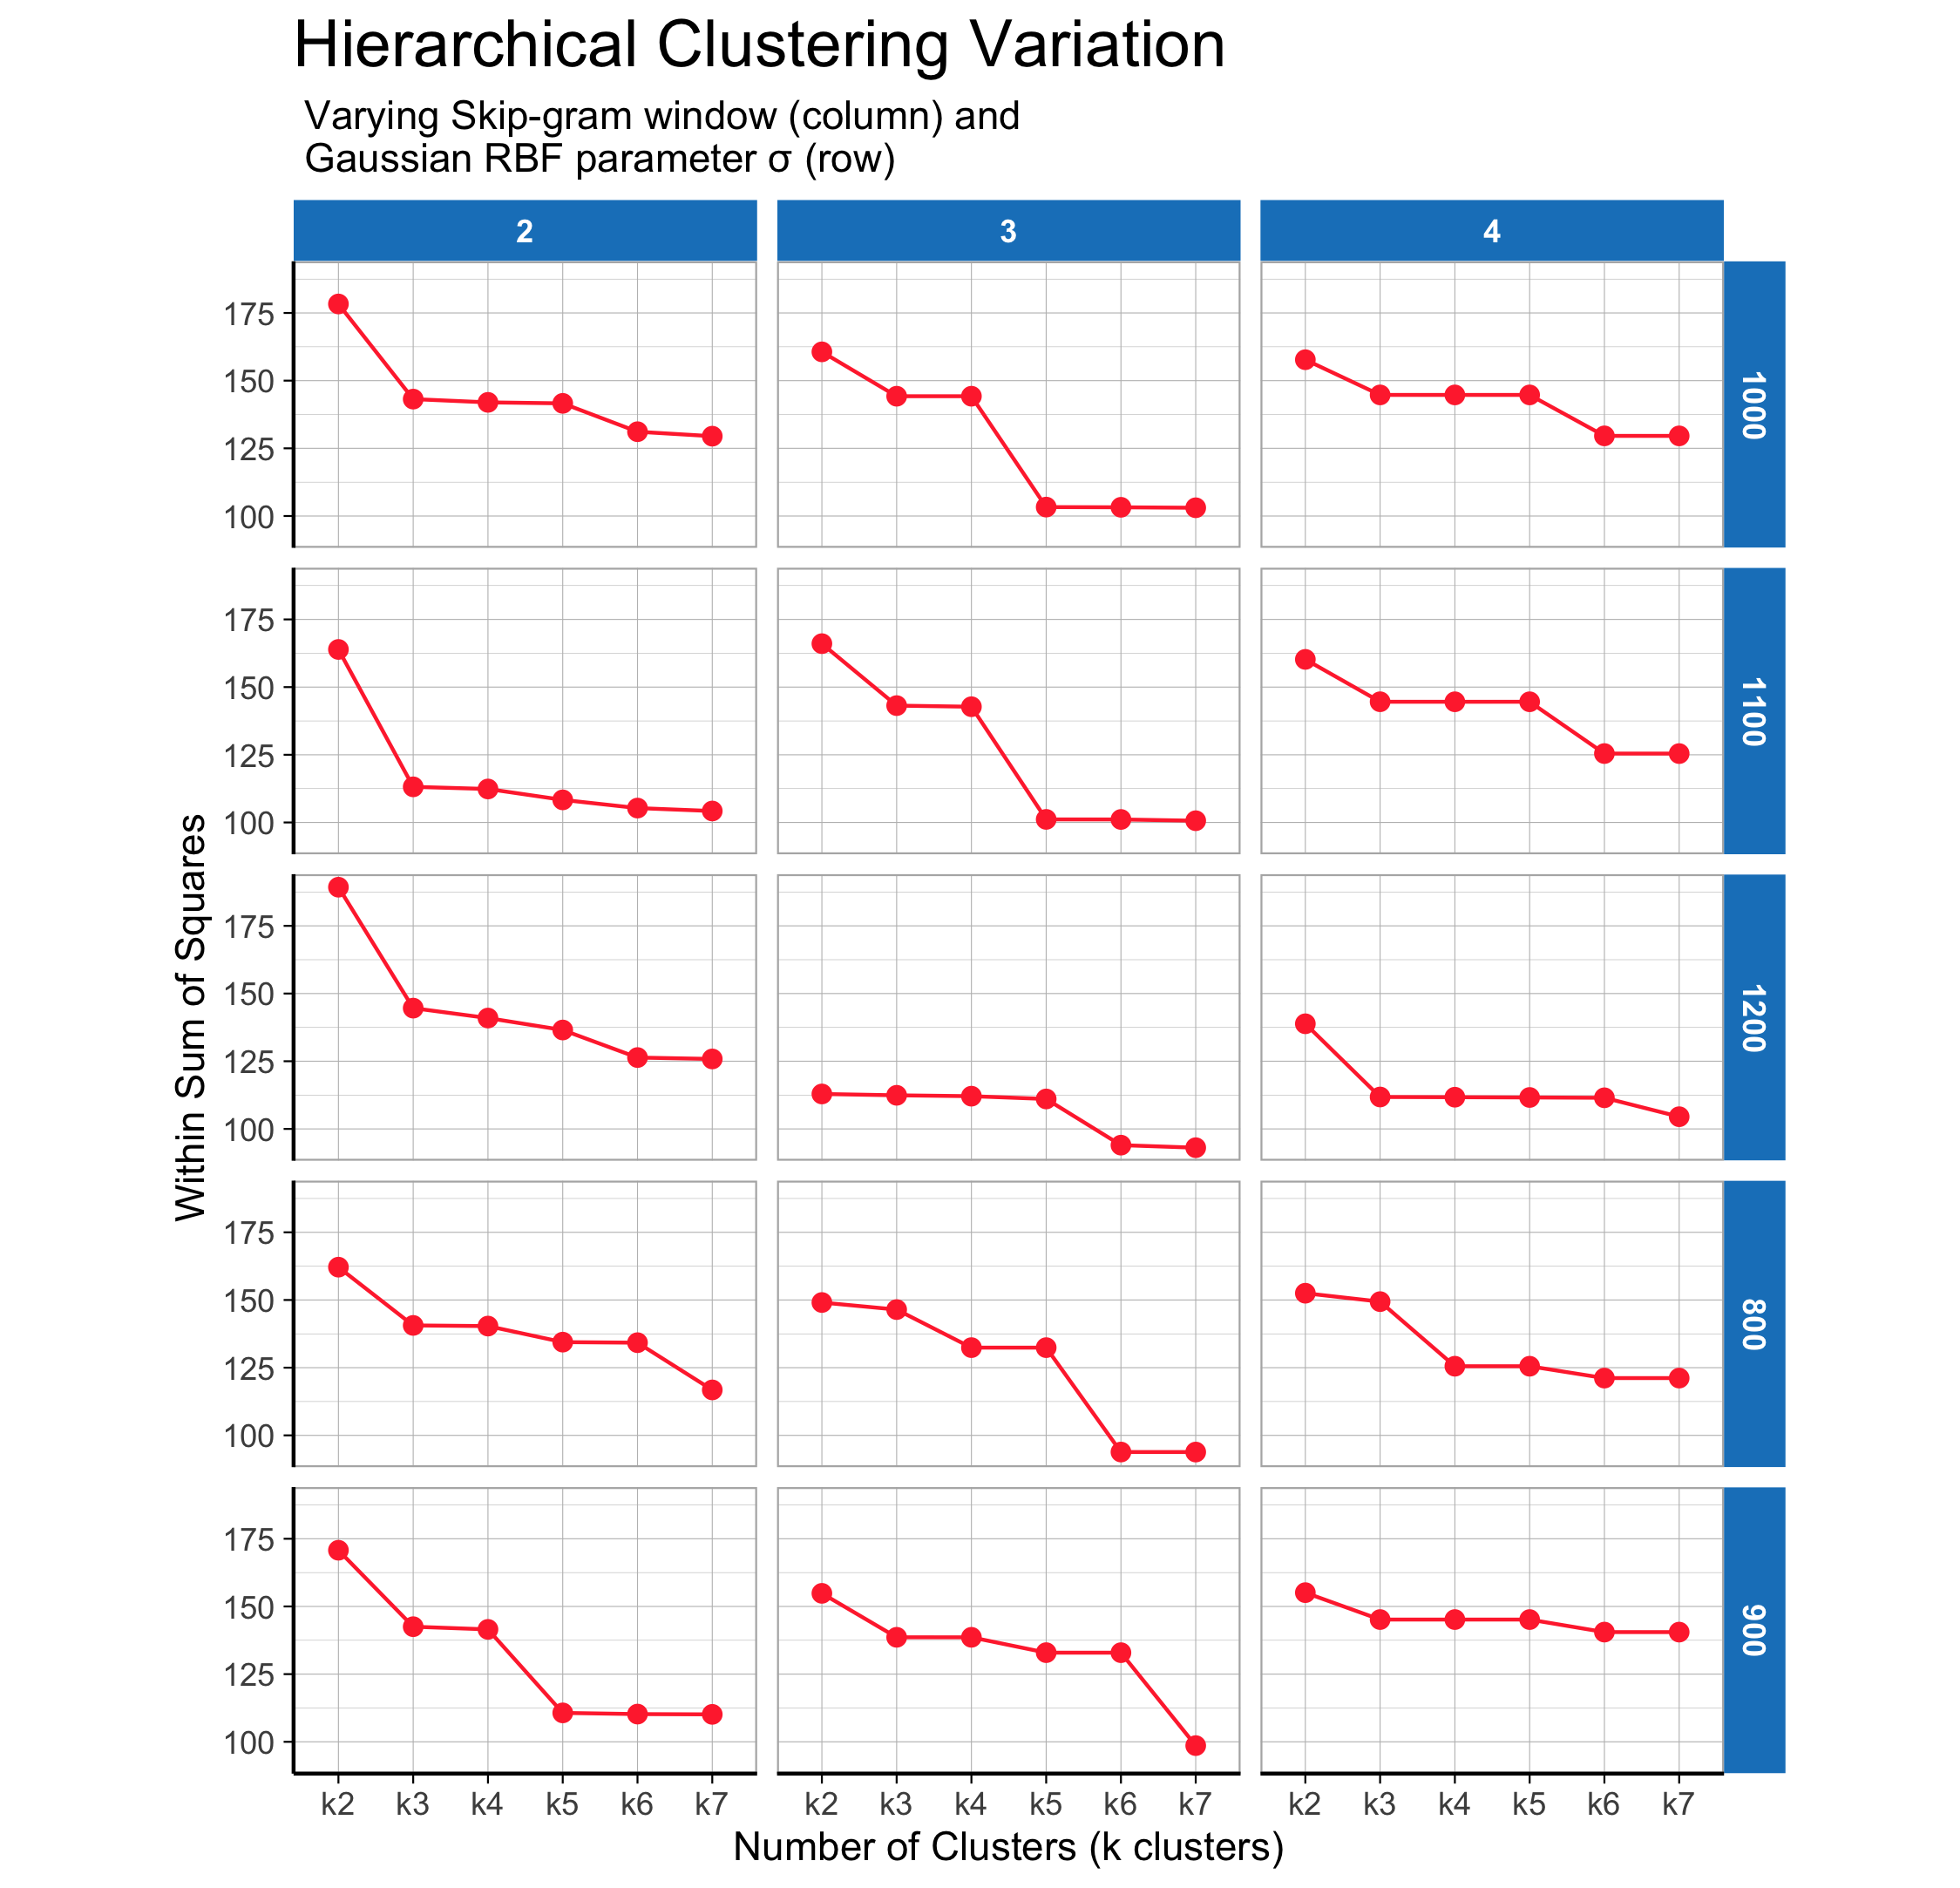
\includegraphics[width=6in]{Content/Images/hclust_variation.png}
\caption{Hierarchical Clustering Variation (NHTSA) for differing hyperparameters.}
\end{figure}

In Figure X, we see some promising values occurring at more prominent ``elbow" points in the plots. These points will be further analyzed and compared. The hyper parameters for these points are:\\

\begin{table}
\begin{tabular}{c|c|c|c}
Point&Skip-gram k& Graph Kernel sigma&No. of Clusters \\
\hline
A&3&1000&5\\
B&2&1100&3\\
C&3&1100&5\\
D&3&800&6\\
E&3&900&7
\end{tabular}
\caption{Hyperparameter for Variation Study in Figure X}
\end{table}

These hyper-parameter sets, and their corresponding graph kernel matrix, are used in a hierarchical clustering analysis. The results from the analysis perform well, and display prominent clusters, often of comparable sizes.In Figure X, we see the 5 dendrograms produced from hyper-parameter sets A,B,C,D, and E. Upon some examination, one will notice that documents often appear in the same clusters together, regardless of the hyper-parameter sets. This is most encouraging, as it indicates that these clusters are not a result of user-chosen parameters, but that the documents are similar. \\

\begin{figure}
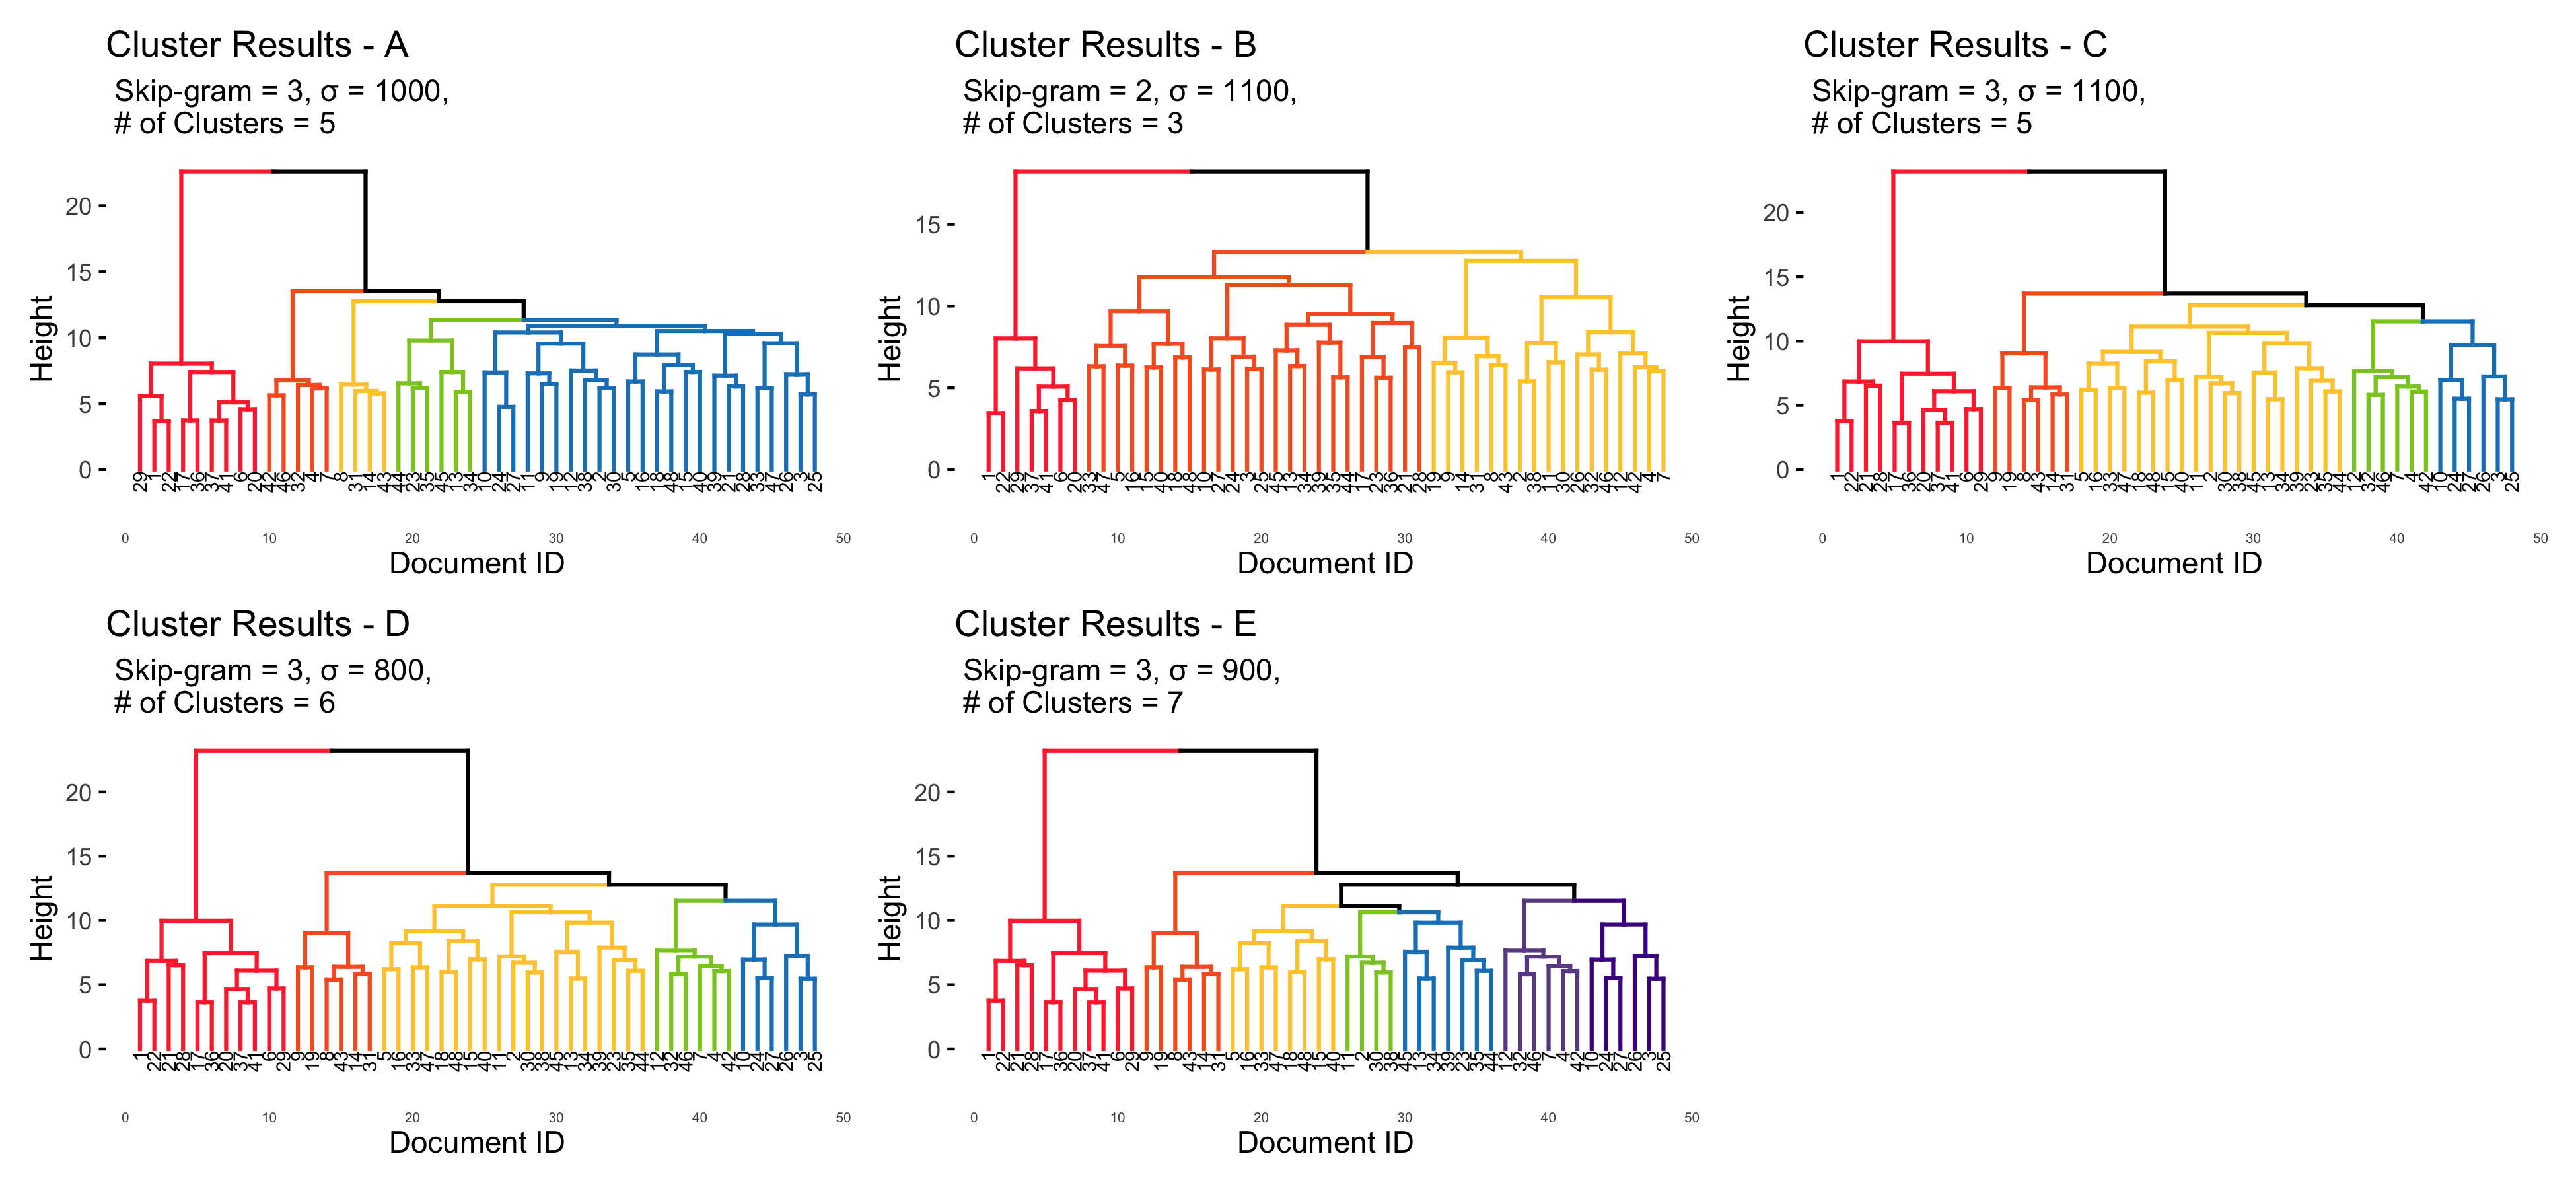
\includegraphics[width=6in]{Content/Images/5cluster.png}
\caption{Five hyper-parameter sets and their corresponding dendrograms.}
\end{figure}

To compare how often this co-membership in groups was appearing, a matrix of co-membership was created. In Figure X, we see that each document has a set of other documents with which it is always clustered with, regardless of hyper-parameter configurations. These small document sets are the document sets which we can expect to have the most in common with one another.\\

\begin{figure}
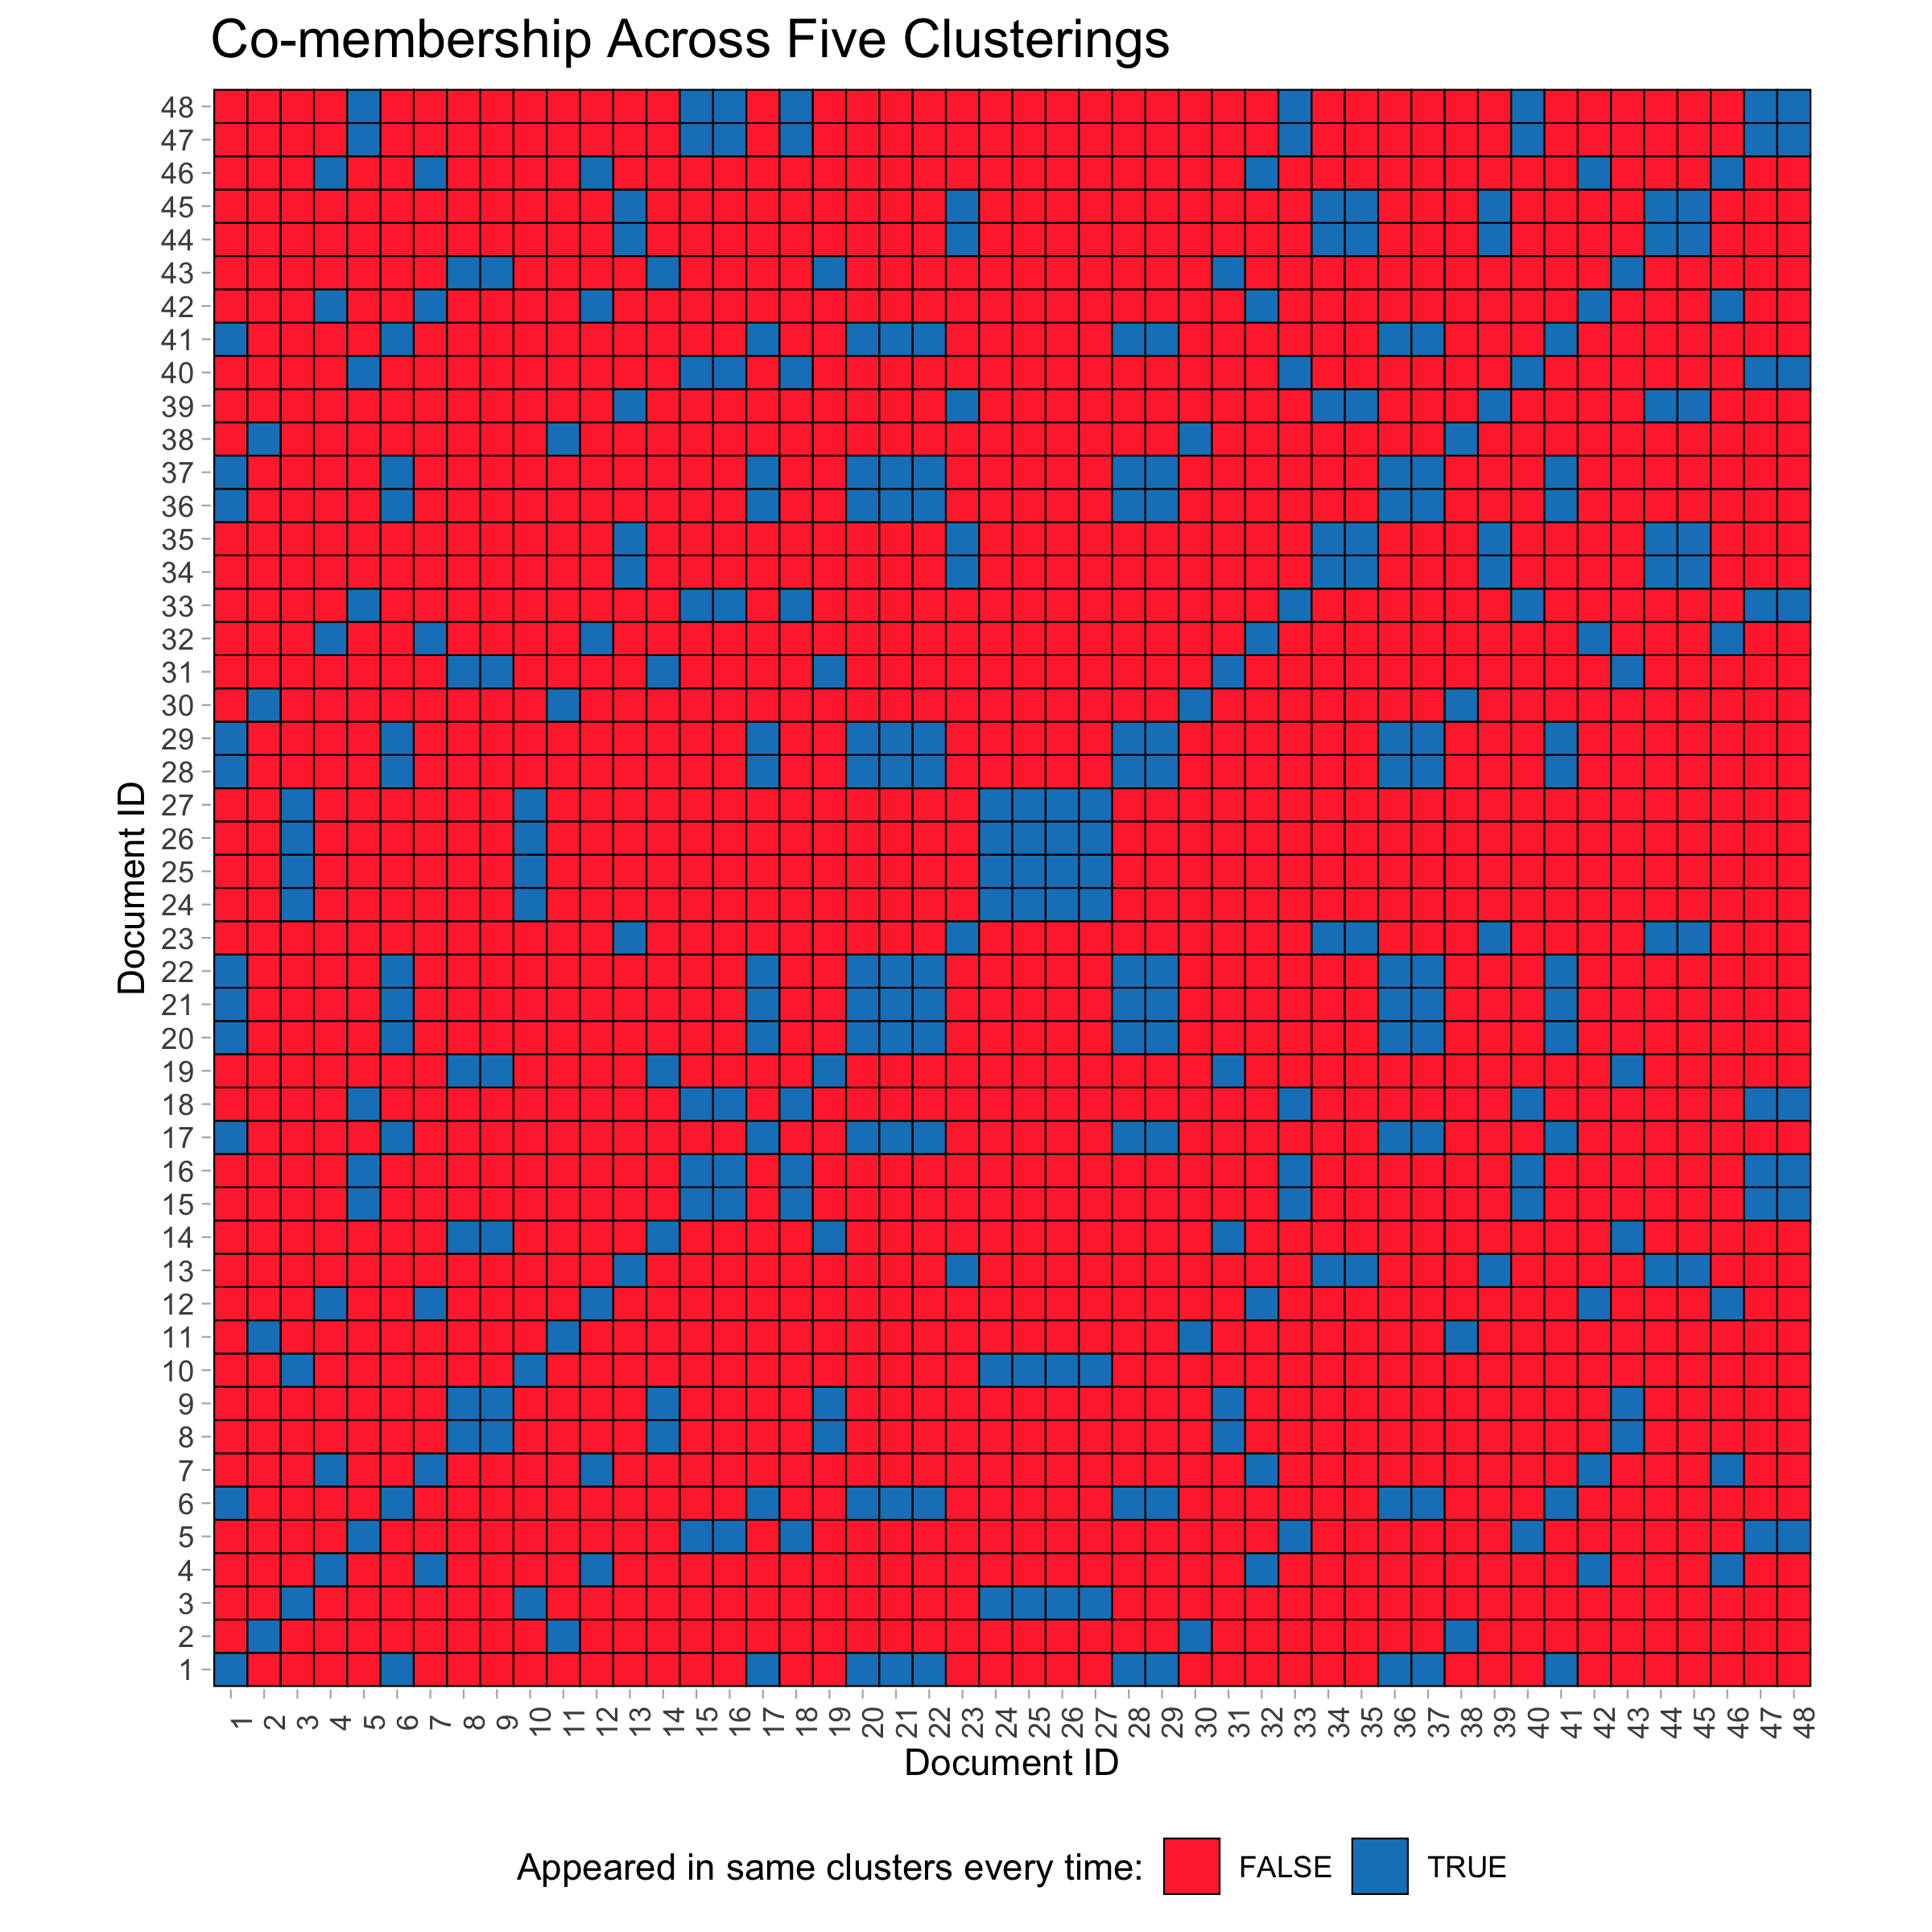
\includegraphics[width=6in]{Content/Images/comembers5.png}
\caption{Co-membership of documents across hyper-parameter sets A,B,C,D, and E.}
\end{figure}

We can inspect the results by checking some of the co-members' text. For example, document two (which was an ambulance crash in Angola, Delaware), has only 3 other co-members. Document two's co-members are: document 11, document 30, and document 38. Document 11 was an ambulance crash in Sheridan, Indiana. Document 30 was an ambulance crash in Pasadena, California. Document 38 was an ambulance crash in Ocilla, Georgia.\\
Now, we can examine some information about these four incidents that may explain their clustering. For example, all of these incidents had fatalities, three of them had roll over events, and these four were all front end collisions to the ambulance where they struck another vehicle, or object, head on. While this is just one example of the clustering methods identifying similarities in the text, we can examine similarities across the dataset through use of term-frequency/inverse document frequency.\\

\begin{figure}
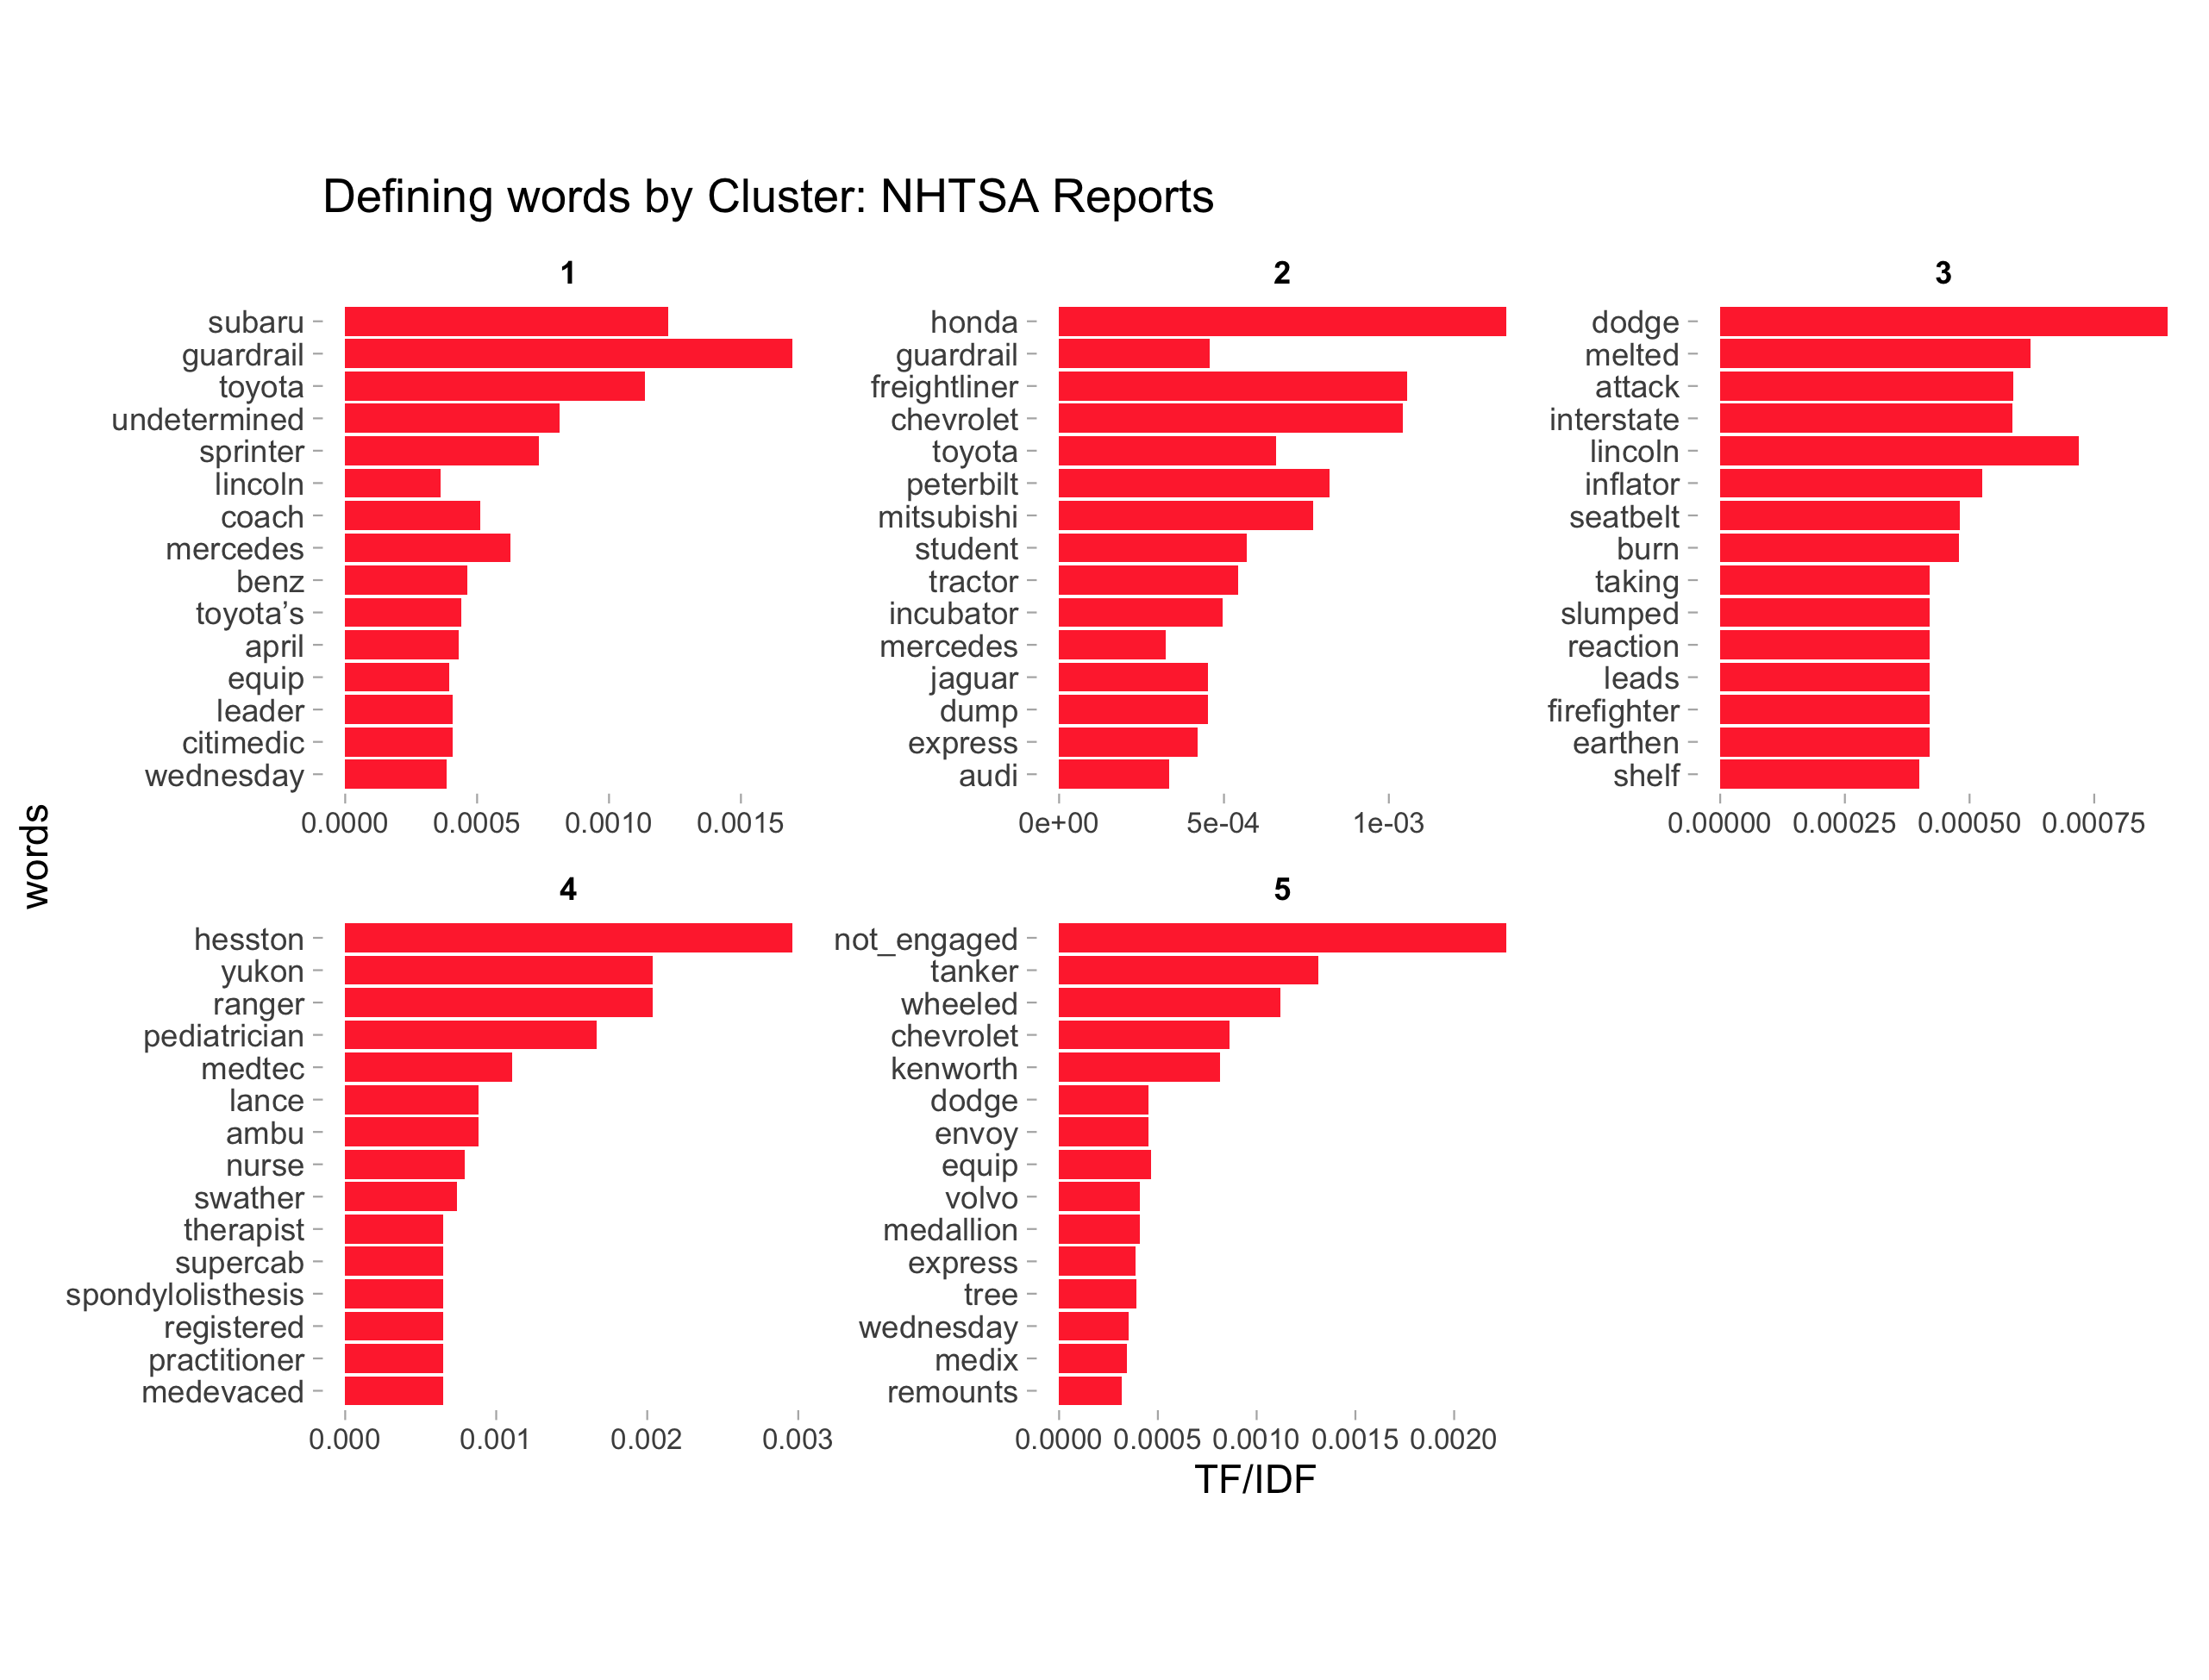
\includegraphics[width=6in]{Content/Images/nhtsa_tf_idf.png}
\caption{Term-Frequency/Inverse Document-Frequency for NHTSA reports, using hyper parameter set A.}
\end{figure}

In Figure 4.4, we see that words that appear frequently, and are unique to that cluster appear to be vehicle manufacturers, medical terms, and words that describe a crash situation (e.g. guardrail, tree, interstate). We can use these to get an idea of the crash situation. Alternatively, we can also examine portions of the skip-gram graph produced, which was used for the graph kernel calculation. \\

\begin{figure}
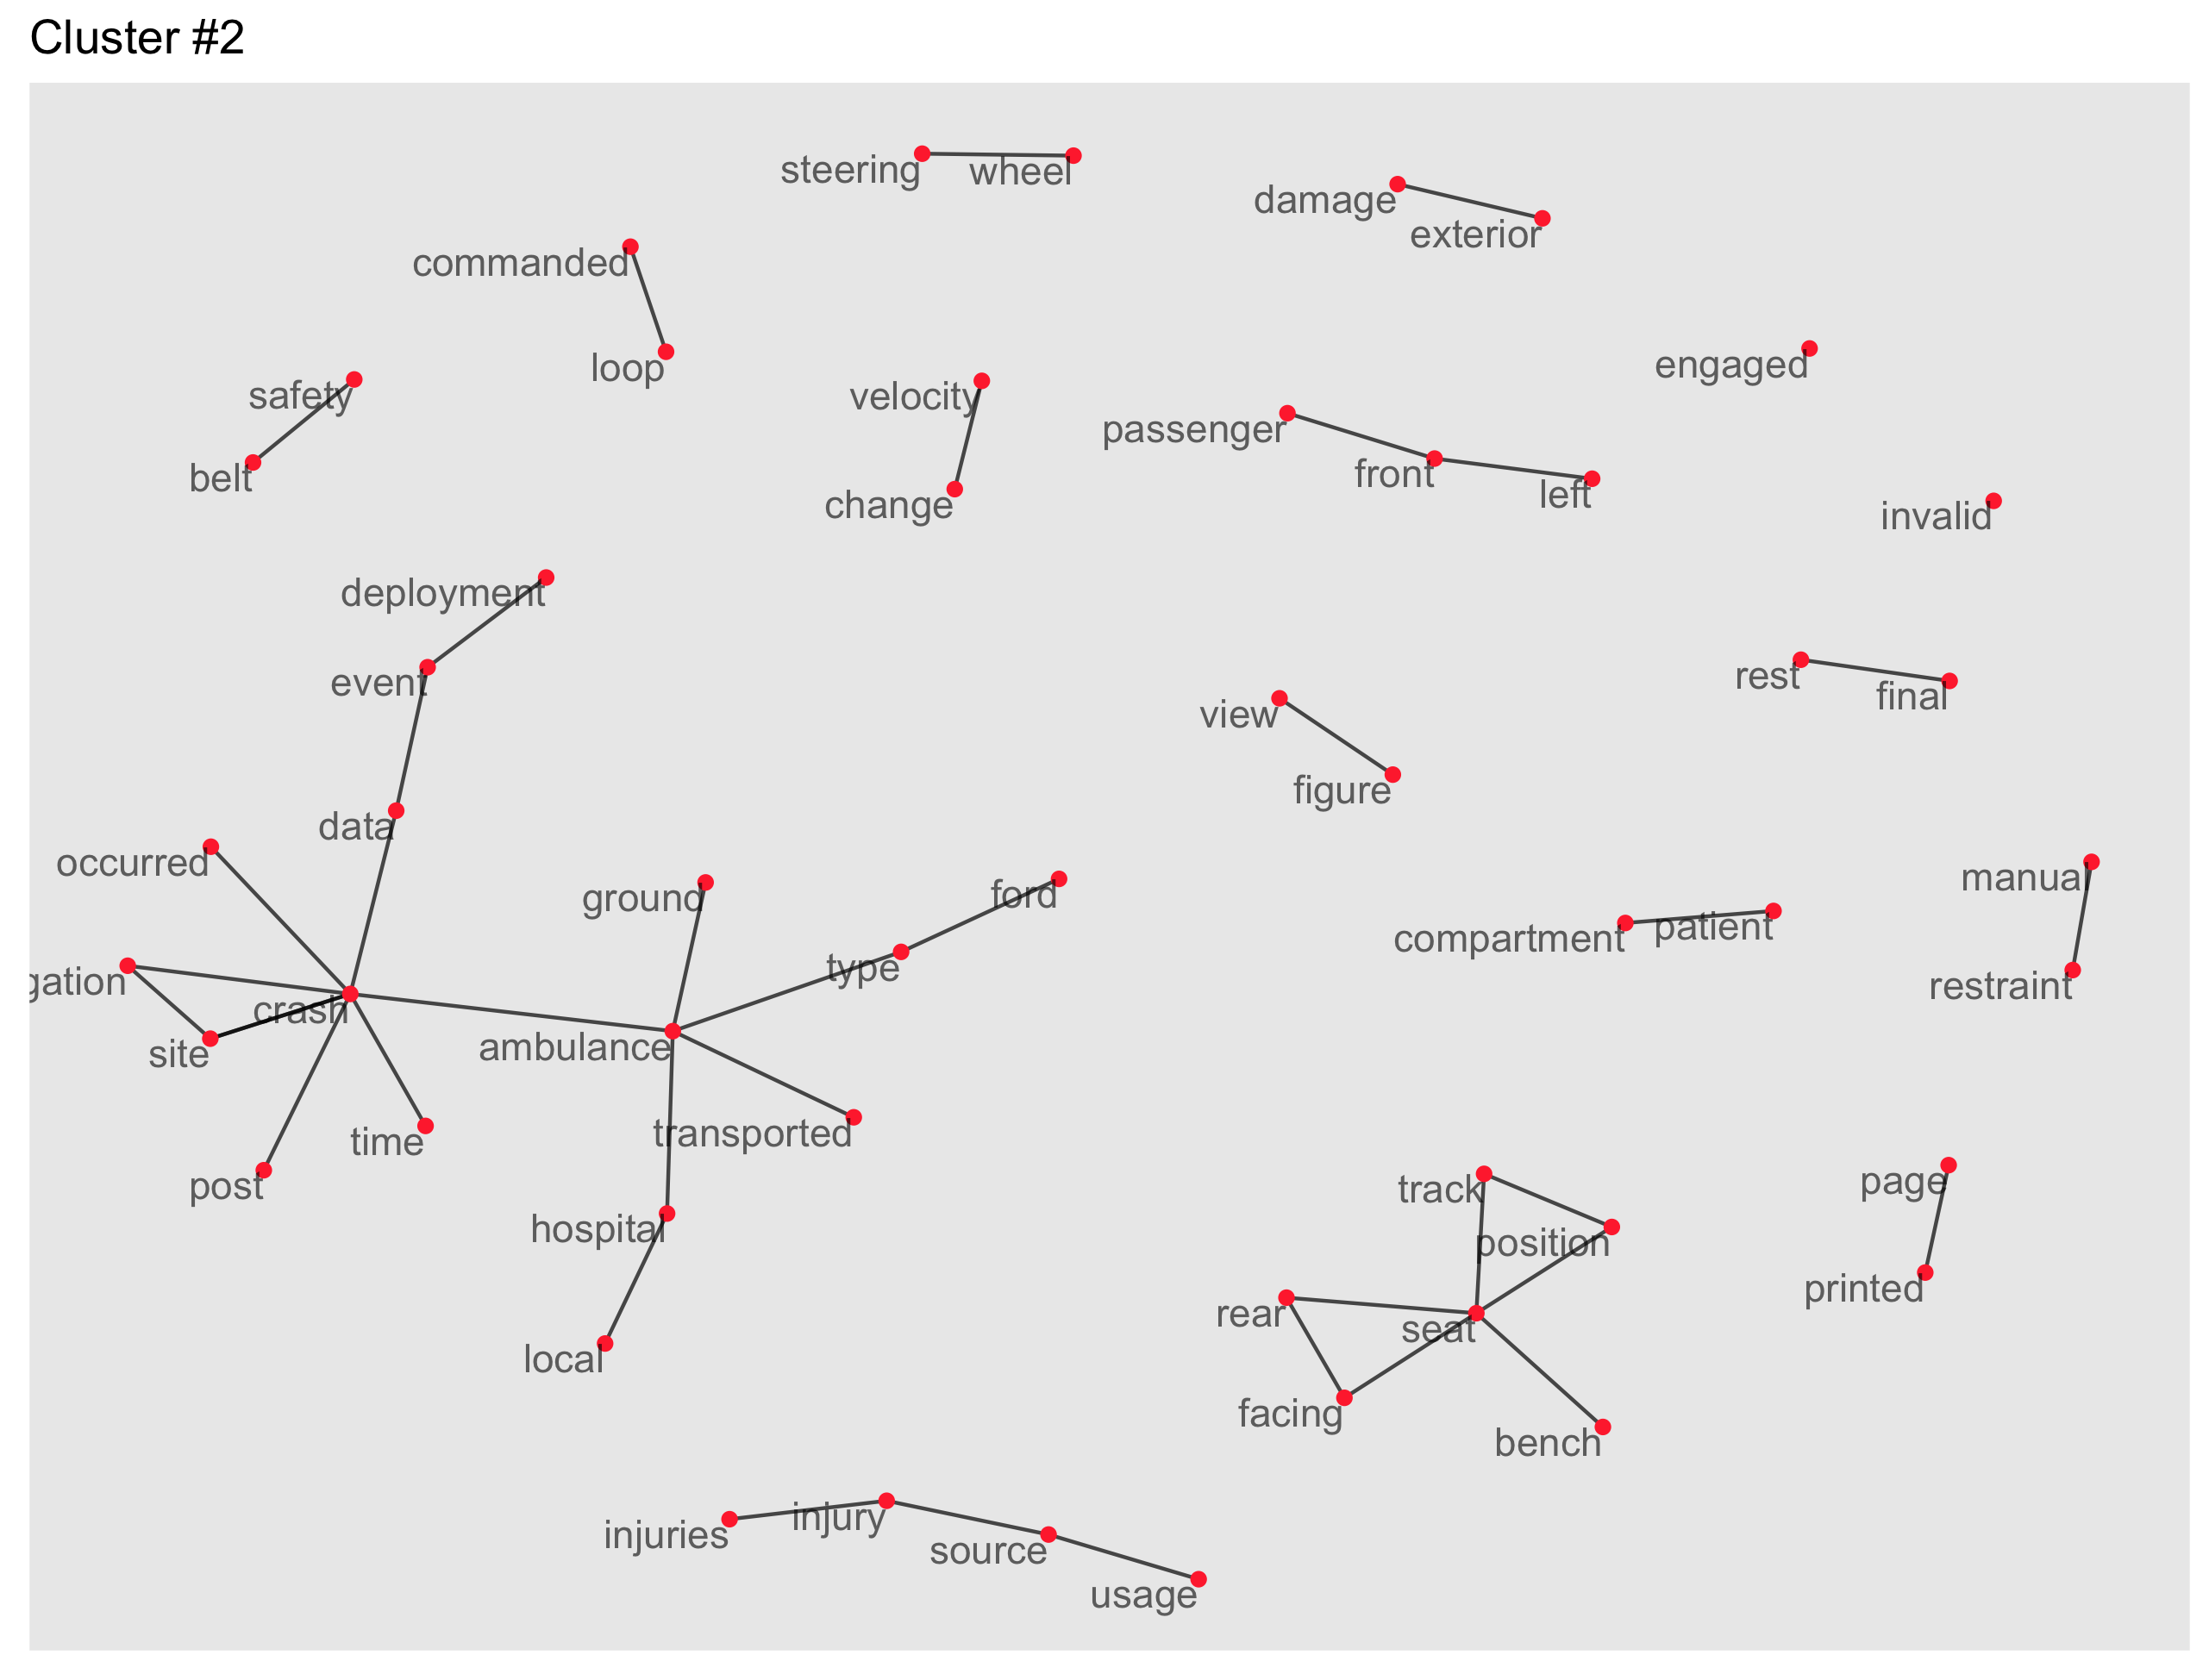
\includegraphics[width=6in]{Content/Images/graph_k5_2.png}
\caption{Skip-grams which occurred more than 50 times in hierarchical clustering with hyper-parameter set A, in cluster 3.}
\end{figure}

We can put together some of the ideas and topics discussed in the cluster. For example, in Figure 4.5 we see that "Front Left Passenger", "Rear Facing Seat", and "Patient Compartment" are all skip-grams which appeared frequently in this cluster.\\


\subsection{reddit Threads}

For the reddit threads dataset, ...\\


\subsection{Comparative Analysis}

Looking at the results from both hierarchical clusterings on the graph kernels...\\
 


